\chapter{Resultados y discusión}

\section{Estabilidad de estructuras}

Antes de estudiar la acidez de los compuestos a proponer, se hace un análisis de la estabilidad de sus isómeros y confórmeros con el fin de buscar las estructuras más estables. 
Se estudiarán los posibles isómeros y confórmeros de los ácidos sulfúrico, carbónico y fosfórico (ANEXO X) con el fin de hallar la estructura más estable en fase gas. \\

  \begin{table}[H]
\begin{center}
\begin{tabular}{|c|c|c|c|c|c|}
\hline
Isómeros $H_2SO_4$ & $\Delta E$ & Isómeros $H_2CO_3$ & $\Delta E$ & Isómeros $H_3PO_4$ & $\Delta E$ \\ \hline
$Conf_1$ & 4,2 & $Conf_1$ & 0,0 & $Conf_1$ & 1,0 \\ \hline
$Conf_2$ & 2,5 & $Conf_2$ & 1,4 & $Conf_2$ & 0,5 \\ \hline
$Conf_3$ & 0,0 & -- & -- & $Conf_3$ & 0,0 \\ \hline
-- & -- & -- & -- & $Conf_4$ & 0,6 \\ \hline
\end{tabular}
\caption{Diferencias de la energía libre de Gibbs en Kcal/mol de cada isómero conformacional de los ácidos.}
\label{tab:3.1}
\end{center}
\end{table}
A la vista de los resultados de energías expuestos en la Tabla 3.1, el isómero más estable del ácido sulfúrico es el confórmero 3, debido a que dicha disposición espacial minimiza las repulsiones de los pares de electrones originando una baja energía y a su vez una mayor estabilidad, ésta también se debe a la posible formación de puentes de hidrógeno intramoleculares, ya que los hidrógenos 3 y 7 de dicho confórmero están dirigidos hacia los átomos de oxígeno 5 y 4 respectivamente, con dos pares de electrones libres en orbitales p, la distancia de los H a los O es menor que la suma de sus radios de Van Der Waals, los H presentan una carga positiva y los oxígenos una negativa como se muestra en la figura 3.1. \\

\begin{figure}[H]
	\centering
	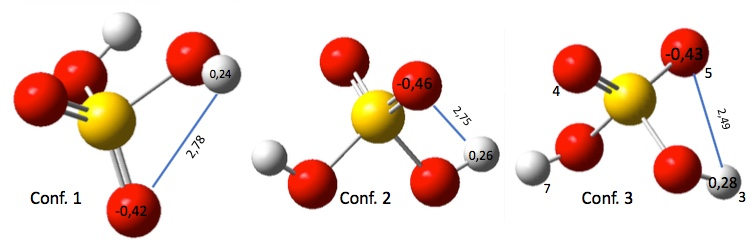
\includegraphics[scale=0.4]{prezimagen}
	\caption{Parámetros para un enlace de hidrógeno, distancias en $\Armstrong$}
\end{figure}

\begin{center} Radios de Van Der Waals en $\Armstrong $
	$$O\longrightarrow1,5$$
	$$H\longrightarrow1,2
	$$
\end{center}

\begin{figure}[H]
	\centering
	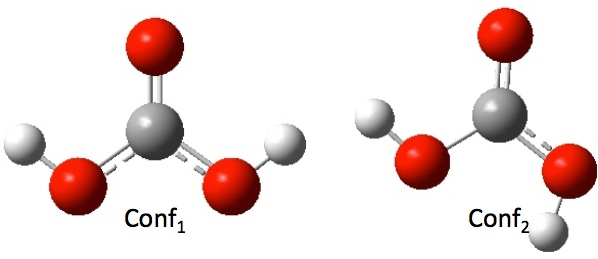
\includegraphics[scale=0.4]{prezimagen4}
	\caption{Confórmeros del $H_2CO_3$.}
\end{figure}
El confórmero del ácido carbónico más estable es el confórmero 1, ver figura 3.2, pero hay que tener en cuenta que la diferencia de energía es mínima, los dos confórmeros presentan una estructura trigonal plana, y un enlace muy fuerte CO. A primera vista, se diría que el confórmero 2 es el más estable debido a a la repulsión electrónica de los pares libres de los dos oxígenos, pero si nos fijamos en la deslocalización electrónica se ve que, los tres enlaces del confórmero 1 son $\pi$, ya que hay resonancia entre los oxígenos de los grupos OH y, en el confórmero 2 hay dos enlaces $\pi$ debido a la resonancia entre un oxigeno del grupo OH y otro del grupo CO, y un enlace $\sigma$ C-OH, por tanto los enlaces del confórmero 1 son más fuertes y la molécula presenta menor energía total y mayor estabilidad, tabla 3.2. 
\begin{table}[H]
    \centering
    \begin{tabular}{|c|c|c|}
    \hline
    Confórmeros del $H_2CO_3$ & $d(C-OH_{(1)})$ & $d(C-OH_{(2)})$ \\ \hline
    $Conf_1$ & 1,340 & 1,340  \\ \hline
    $Conf_2$ & 1,360 & 1,340 \\ \hline 
    \end{tabular}
    \caption{Distancias C-OH del ácido carbónico}
\end{table}

En cuanto a los confórmeros del ácido fosfórico, no se puede decir que el confórmero 3 sea el más estable ya que las diferencias de energía son demasiado pequeñas, y entra dentro del error que puede tener el método teórico usado. Ver tabla \ref{tab:3.1}. Esto es debido a que las cuatro distancias P-O de los confórmeros son relativamente altas y no hay posibilidad de formación de enlaces de hidrógeno para ninguna de las estructuras propuestas.

Se estudia también la estabilidad de los isómeros y confórmeros de los ácidos anteriores sustituyendo uno o varios átomos de hidrógeno por halógenos. Tablas de la 3.3 a la 3.6. Al sustituir un átomo de hidrógeno por un halógeno la distribución de carga de la molécula se verá afectada, y por tanto, la disposición espacial de los átomos, el halógeno podrá asociarse tanto al átomo central como a uno de los oxígenos. Una de las ideas propuestas derivadas de este estudio de  estabilidad, es localizar la estructura más favorable para conseguir evaluar el efecto de la sustitución sobre la acidez. Ver estructuras de todos los isómeros considerados en el ANEXO X.

\begin{figure}[H]
	\centering
	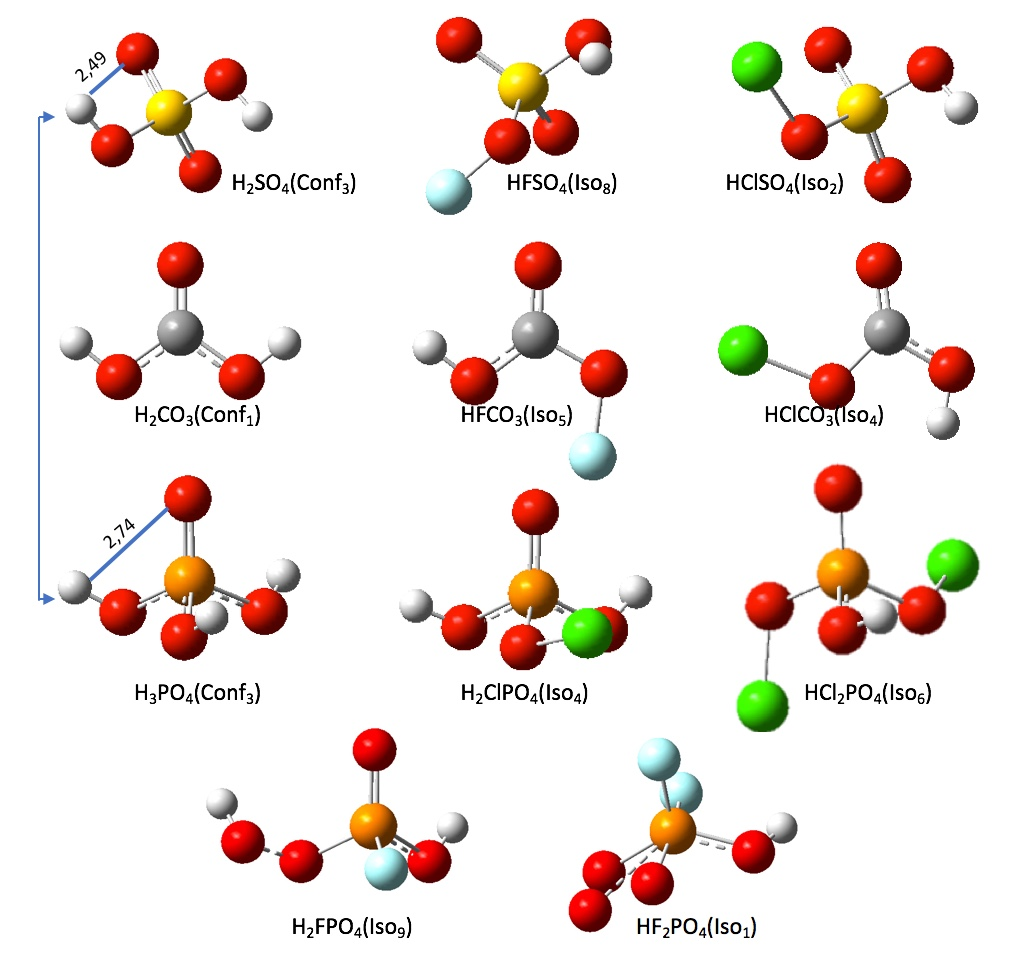
\includegraphics[scale=0.3]{prezimagen2}
	\caption{Isómeros más estables de los ácidos objeto de estudio.}
\end{figure}

En primer lugar se estudian los isómeros y confórmeros del ácido sulfúrico sustituido, donde el isómero 2 del $HClSO_4$ tiene dos enlace S-O muy fuerte (d(S-O)=1,43$\Armstrong$) y la disposición del cloro es tal que no hay impedimento estérico ya que está en trans con el hidrógeno. (Ver Fig 3.4 \emph{$HClFSO_4(iso_2)$}). El isómero 8 del $HFSO_4$ es la molécula más estable (Ver Fig 3.4 \emph{$HFSO_4(iso_8)$}) en la sustitución de un hidrógeno por un átomo de flúor, ya que es la única con dos enlaces S-O muy fuertes (d(S-O)=1,43 $\Armstrong$), además sienten mucha atracción ya que el azufre tiene gran carga natural positiva y los dos oxígenos gran carga negativa (S=2,39 y cada uno de los oxígenos de dicho enlace fuerte -0,81). 

\begin{table}[H]
	\begin{center}
		\begin{tabular}{|c|c|c|c|}
			\hline
			Isómeros $HFSO_4$ & $\Delta E$ & Isómeros $HClSO_4$ & $\Delta E$ \\ \hline
			$iso_1$	& 10,8 & $iso_1$ & 0,1 \\ \hline
			$iso_2$ & 10,8 & $iso_2$ & 0,0 \\ \hline
			$iso_3$ & 10,8 & $iso_3$ & 65,0 \\ \hline
			$iso_4$ & 10,8 & $iso_4$ & 64,2 \\ \hline
			$iso_5$ & 42,7 & $iso_5$ & 24,4 \\ \hline
			$iso_6$ & 10,8 & $iso_6$ & 0,1 \\ \hline
			$iso_7$ &	101,3 & $iso_7$ & 110,0 \\ \hline
			$iso_8$ &	0,0 & $iso_8$ & 4,8 \\ \hline
		\end{tabular}
		\caption{Diferencias de la energía libre de Gibbs en Kcal/mol de cada isómero conformacional del ácido sulfúrico sustituyendo un H por un halógeno}
	\end{center}
\end{table}

Los isómeros más estables del ácido carbónico sustituido con halógenos presentan distancias menores de enlaces C-O, dos isómeros de cada compuesto halogenado presentan hibridación $sp^2$, es decir, enlaces más fuertes, por ello la diferencia entre los isómeros 4 y 5 es tan pequeña, en el caso del compuesto de flúor la diferencia es de de 2 Kcal/mol esto puede ser porque el enlace de hidrógeno que se forma es más débil en el isómero 4, debido a la proximidad del flúor al oxígeno que interviene y por consiguiente, una carga menos negativa de éste. Véase la figura 3.3.

\begin{figure}[H]
	\centering
	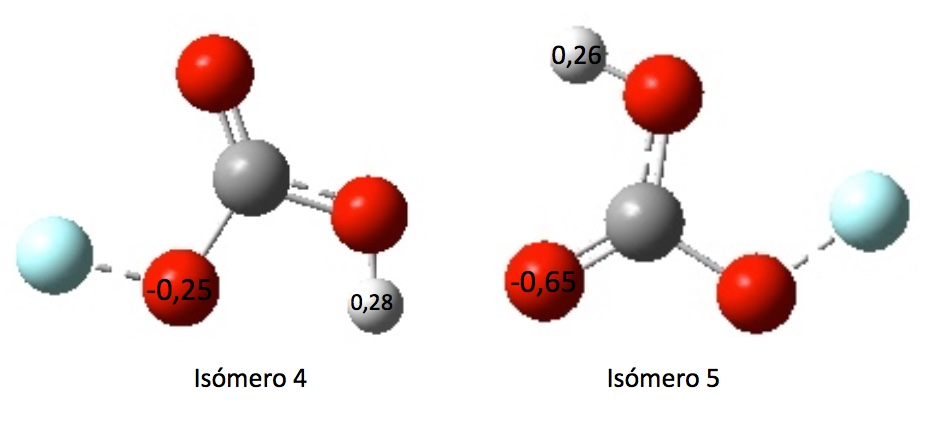
\includegraphics[scale=0.2]{prezimagen3}
	\caption{Isómeros $HFCO_3$}
\end{figure} 

\begin{table}[H]
	\begin{center}
		\begin{tabular}{|c|c|c|c|}
			\hline 
			Isómeros $HFCO_3$ & $\Delta E$ & Isómeros $HClCO_3$& $\Delta E$ \\ \hline
			$Iso_1$ & 4,0 & $Iso_1$ & 49,9 \\ \hline
			$Iso_2$ & 3,9 & $Iso_2$ & 49,0 \\ \hline
			$Iso_3$ & 92,7 & $Iso_3$ & 92,0 \\ \hline
			$Iso_4$ & 1,8 & $Iso_4$ & 0,0 \\ \hline
			$Iso_5$ & 0,0 & $Iso_5$ & 0,3 \\ \hline
		\end{tabular}
		\caption{Diferencias de la energía libre de Gibbs en Kcal/mol de cada isómero conformacional del ácido carbónico sustituyendo un hidrógeno por un halógeno}
	\end{center}
\end{table}

Análogamente a los casos de los ácidos anteriores se concluye que los compuestos más estables al sustituir un hidrógeno por un halógeno en el ácido fosfórico son el isómero 9 en el caso del $H_2FPO_4$ y en el de $H_2ClPO_4$ el Isómero 3 (Figura 3.4), la estabilidad de éstos se debe a su geometría tetraédrica, hibridación $sp^3$, los isómeros restantes con dicha estructura son los que no presentan gran diferencia energética (isómeros 1, 2 y 3 para el compuesto con flúor e isómeros 1, 2, 11 y 12 para el de cloro), no es posible explicar la estabilidad del isómero comparada con éstos ya que tenemos que tener en cuenta el error del cálculo computacional. 

\begin{table}[H]
\begin{center}
\begin{tabular}{|c|c|c|c|}
\hline
Isómeros $H_2FPO_4$ & $\Delta E$ & Isómeros $H_2ClPO_4$ & $\Delta E$ \\ \hline
$Iso_1$& 1,3 & $Iso_1$ & 0,9 \\ \hline
$Iso_2$ & 1,3 & $Iso_2$ & 0,9 \\ \hline
$Iso_3$ & 0,01 & $Iso_3$ & 0,0 \\ \hline
$Iso_4$	& 8,6 & $Iso_4$ & 40,0 \\ \hline
$Iso_5$	& 8,6 & $Iso_5$ & 40,0 \\ \hline
$Iso_6$	& 56,7 & $Iso_6$ & 29,1 \\ \hline
$Iso_7$	& 8,4 & $Iso_7$ & 40,7 \\ \hline
$Iso_8$	& 8,6 & $Iso_8$ & 43,5 \\ \hline
$Iso_9$	& 0,0 & $Iso_9$ & 30,0 \\ \hline
$Iso_{10}$	& 57,9 & $Iso_{10}$ & 90,2 \\ \hline
$Iso_{11}$ & 22,2 & $Iso_{11}$ & 1,3 \\ \hline
$Iso_{12}$ & 23,2 & $Iso_{12}$ & 0,5 \\ \hline
\end{tabular}
\caption{Diferencias de la energía libre de Gibbs en Kcal/mol de cada isómero conformacional del ácido fosfórico sustituyendo un hidrógeno por un halógeno.}
\end{center}
\end{table}

Por último, al sustituir un hidrógeno más por otro halógeno las moléculas de mayor estabilidad son el isómero 1 para el  $HF_2PO_4$, ésto es debido a que es el único isómero que forma un enlace de hidrógeno con el flúor (d(H--F)=2,2$\Armstrong$), en el caso del  $HCl_2PO_4$ el isómero 6, hay que tener en cuenta que hay dos isómeros más de esta última molécula muy parecidos en energía, son las únicas con geometría tetraédrica, en el caso del isómero 6, no hay tanto impedimento estérico por parte de los átomos de cloro, traduciéndose ésto en una mayor estabilidad de la molécula. 

\begin{table}[H]
	\centering
	\begin{tabular}{|c|c|c|c|}
		\hline
		Isómeros $HF_2PO_4$ & $\Delta E$   & Isómeros $HCl_2PO_4$ & $\Delta E$     \\ \hline
		$Iso_1$  & 0,0     & $Iso_1$     & 98,7 \\ \hline
		$Iso_2$  & 18,0    & $Iso_2$   & 38,5 \\ \hline
		$Iso_3$   & -- & $Iso_3$    & 39,3 \\ \hline
		$Iso_4$   & --& $Iso_4$    & 39,3 \\ \hline
		$Iso_5$   & -- & $Iso_5$  & 38,5 \\ \hline
		$Iso_6$    & 60,6    & $Iso_6$  & 0,0  \\ \hline
		$Iso_7$   & 60,6    & $Iso_7$   & 2,1  \\ \hline
		$Iso_8$    & 15,9    & $Iso_8$  & 19,5 \\ \hline
		$Iso_9$   & 36,5    & $Iso_9$   & 0,1  \\ \hline
		$Iso_{10}$  & 39,1    & $Iso_{10}$   & 38,7 \\ \hline
	\end{tabular}
\caption{Diferencias de la energía libre de Gibbs en Kcal/mol de cada isómero conformacional del ácido fosfórico sustituyendo dos hidrógenos por dos halógenos.}
\end{table}

Si se observa la tabla 3.6, el vacío de los isómeros 3, 4 y 5 del $HF_2PO_4$ se debe a que las geometrías propuestas no se optimizaron ya que no se llegó a un mínimo de energía.


\begin{comment}También se ha realizado el estudio de estabilidad entre dichos ácidos observando el isómero más estable de cada uno, ver tabla 3.7, se tiene que el ácido más estable es el sulfúrico, seguido del fosfórico y por último, el menos estable de los tres, el ácido carbónico \\

\begin{table}[H]
	\centering
	\begin{tabular}{|c|c|c|c|c|c|}
		\hline
Ácido&$\Delta E$&Ácido&$\Delta E$& Ácido&$\Delta E$\\ \hline
$H_2SO_4$&0,00&$HFSO_4$&0&$HClSO_4$&0\\ \hline
$H_3PO_4$&3,52E+04&$H_2FPO_4$&3,52E+04&$H_2ClPO_4$&3,52E+04\\ \hline
$H_2CO_3$&2,73E+05&$HFCO_3$&2,73E+05&$HClCO_3$&2,73E+05\\ \hline
	\end{tabular}
	\caption{Diferencias de energía en Kcal/mol}
\end{table}
Dicha estabilidad se debe a que la estructura del ácido carbónico es plana (trigonal plana) y por lo tanto más rígida, lo que le proporciona menor estabilidad.\\ Sin embargo, las otras dos estructuras son tetraédricas, en el caso del ácido fosfórico, las distancias P-O son mayores que las distancias S-O, ya que el fósforo es de mayor tamaño que el azufre y menos electronegativo, por consiguiente, distancias O--H mayores, sin posibilidad de formar enlaces de hidrógeno en dicha molécula, mientras que en el ácido sulfúrico si se forma dicho enlace. Ver figura 3.3
\end{comment}

\section{Acidez en fase gas}


La acidez en fase gaseosa de un ácido neutro HA se refiere al siguiente equilibrio:

$$HA\xrightleftharpoons{\Delta G} H^+ + A^-$$

Donde $\Delta G$ es la acidez en fase gaseosa, dicha cantidad es de interés fundamental y proporciona informacion valiosa sobre las propiedades intrínsecas, independientes del disolvente de los ácidos. \cite{quimica3}

Con el fin de estudiar el impacto de las sustituciones de hidrógenos por halógenos en la acidez en fase gas de los ácidos, se han diseñado más estructuras sustituyendo hidrógenos por flúor. Para calcular la acidez en fase gas se han hecho los mismos cálculos computacionales con sus aniones.


 \begin{table}[H]
     \centering
     \begin{tabular}{|c|c|c|c|}
     \hline
     \multicolumn{4}{|c|}{\bfseries{ACIDEZ}} \\ \hline
     Ácido & $\Delta G$ & $\Delta G_{exp}$ & $\Delta G_{ H. especf}$ \\ \hline
$CF_3COOH$ & 314,0 & 316,3 & 309,0\\ \hline
$CF_3COSH$ & 311,6 & 312,5 & 303,4\\ \hline
$CF_3SO_3H$ & 292,9 & 299,5 &292,3\\ \hline
$FHSO_3$ & 293,6 & 299,8 & 293,1\\ \hline
$H_2CFCOOH$ & 328,1 &-- & 320,6\\ \hline
$H_2CFCOSH$ & 324,0 & --& 314,5\\ \hline
$H_2CFSO_3H$ & 303,6 & -- & 302,9\\ \hline
$H_2CO_3$ & 328,0	& -- & 319,7\\ \hline
$H_2S_2O_6$ & 281,8 & -- & 283,4\\ \hline
$H_2SO_4$ & 302,6	& 302,2 & 301,3\\ \hline
$H_3CCOOH$ & 338,6 & -- &	328,9\\ \hline
$H_3CCOSH$ & 330,5 & -- &	319,5\\ \hline
$H_3CSO_3H$ & 312,7 & 315,0 & 309,7\\ \hline
$HCF_2COOH$ & 	321,4 & -- & 315,0\\ \hline
$HCF_2COSH$ & 	316,8 & -- & 308,6\\ \hline
$HCF_2SO_3H$ & 	297,9 & -- & 298,4\\ \hline
$HPO_3$ & 303,5 & 303,3 & 300,9\\ \hline
$HNO_3$ & 315,0 & 317,8 & 309,5\\ \hline
$H_3PO_4$ & 321,4	& -- & 332,6 \\ \hline
$H_2FPO_4$ & 329,3 & -- &\\ \hline
$HF_2PO_4$ & 385,7 & -- &  \\ \hline
$H_2ClPO_4$ & 337,0 & -- &\\ \hline
$HCl_2PO_4$ & 332,2 & -- &\\ \hline
$HFSO_4$ & 283,0 & -- & 285,0 \\ \hline
$HClSO_4$ & 293,3 & -- & 288,5\\ \hline
$HFCO_3$ & 309,1 & -- &\\ \hline
$HClCO_3$ & 312,5 & -- &\\ \hline


     \end{tabular}
     \caption{Acideces en fase gas con y sin hidratación específica y el valor experimental en Kcal/mol. $\cite{quimica3}$ }
     \label{tab:3.7}
 \end{table}

Se han estudiado distintos tipos de ácidos, por un lado, los oxácidos estudiados en la parte 1 del presente trabajo añadiendo alguno más y, por otro lado, algunos ácidos orgánicos de interés, así se hace un estudio de acidez en fase gaseosa más extenso y riguroso.
 
 Los resultados dados en la Tabla 3.7 apoyan el siguiente orden de acidez intrínseca para los ácidos orgánicos: $ CF_3SO_3H>HCF_2SO_3H>H_2CFSO_3H>CF_3COSH>H_3CSO_3H>CF_3COOH>HCF_2COSH>HCF_2COOH>H_2CFCOSH>H_2CFCOOH>H_3CCOSH>H_3COOH $, y el siguiente para los oxácidos: $ H_2S_2O_6>FHSO_3>H_2SO_4>HPO_3>HNO_3>H_3PO_4>H_2CO_3 $.

Los ácidos llamados normalmente fuertes ($ CF_3SO_3H$, $FHSO_3$, $HCF_2SO_3H$, $H_2SO_4$, $HPO_3$, $H_2CFSO_3H$) están en un intervalo de acidez relativamente estrecho (10,7 kcal/mol), se tienen algunos valores experimentales, donde la variación con los calculados computacionalmente no llega a las 3 Kcal/mol exceptuando al $CF_3SO_3H$ y al $FHSO_3$ que difieren de 6-7 kcal/mol, al tener una diferencia tan alta, se ha llevado a cabo un cálculo G4 para estos dos últimos ácidos con el fin de ver si el primer cálculo sobreestima la acidez de dichos ácidos. 
\begin{table}[H]
	\centering
	\begin{tabular}{|c|c|c|}
		\hline
		Ácido & $\Delta G$ & $\Delta G_{exp}$ \\ \hline
		$CF_3SO_3H$ & 291,9 & 299,5 \\ \hline
		$FHSO_3$ & 294,8 & 299,8 \\ \hline 
	\end{tabular}
\caption{Acideces en fase gas con el método G4 en Kcal/mol}
\end{table}

En vista de los resultados obtenidos con el método compuesto G4 se observa como la acidez no varía prácticamente nada (1,5Kcal/mol) en comparación con el cálculo DFT, pero podemos decir que dicho método sobreestima la acidez del compuesto inórgánico y subestima la del ácido orgánico y, como era de esperar, el método G4 describe mejor su acidez que el método DFT B3LYP/6-311G**.

La acidez es proporcional a la tendencia del ácido a perder un protón. Se ve como el orden de acidez sustituyendo el grupo ácido es $ COOH {<} COSH {<} SO3H $, ya que en los aniones correspondientes se debe tener en cuenta la estabilización por resonancia, deslocalización de enlaces $\pi$ (figura 3.6), que es mayor en el $SO3^-$ ya que hay mayor número de átomos, en cuanto a las otras dos estructuras, los iones $COS^-$ y $COO^-$ son estabilizados por resonancia, pero en el $COS^-$ es mayor, se puede explicar observando la carga natural en dichos átomos dada en la tabla 3.9. Ver figura 3.5.

\begin{figure}[H]
	\centering
	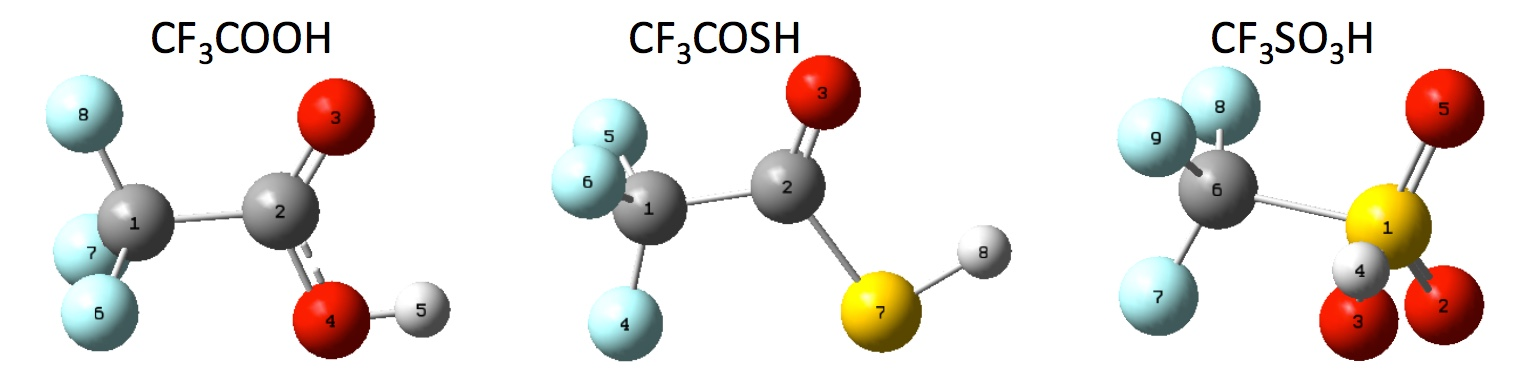
\includegraphics[scale=0.2]{CF3-grupo}
	\caption{Ácidos con tres átomos de flúor}
\end{figure}

\begin{table}[H]
    \centering
    \begin{tabular}{|c|c|c|c|c|c|}
    \hline
    $SO3^-$ & Carga Natural &$COS^-$ & Carga Natural & $COO^-$ & Carga Natural \\ \hline
    S & 2.21439 & C & 0.22678 & C & 0.68743 \\ \hline
    O & -0.97579 & O & -0.61533 & O & -0.73587 \\ \hline
    O & -0.97575 & S & -0.48786 & O & -0.74097 \\ \hline
    O & -0.97579 & -- & -- & -- & -- \\ \hline
    \end{tabular}
    \caption{Cargas naturales de la moléculas $CF_3-$ grupo ácido}
\end{table}

\begin{figure}[H]
\centering
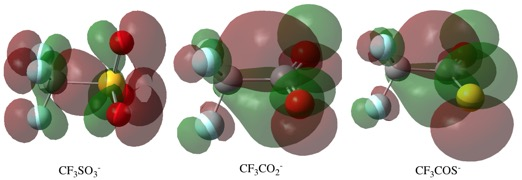
\includegraphics[scale=0.8]{HOMOOrbitale}
\caption{Orbitales moleculares HOMO.}
\end{figure}

Comparamos también sustitución de átomos de flúor por átomos de hidrógeno en el grupo $CF_3$ de la molécula. En la tabla \ref{tab:3.8} se ve que cuantos más átomos de flúor haya en la molécula mayor es su acidez, esto se debe a la elevada electronegatividad del flúor, cuántos más átomos de flúor haya, mayor capacidad atractora tendrá el grupo, y mayor será el efecto inductivo, polarización de carga transmitida por enlaces $\sigma$, si se observan los máximos de densidad en el enlace O-H de cada molécula, (figura 3.8) y las cargas naturales de dichos átomos (tabla 3.10) se comprueba la facilidad de romper dicho enlace en presencia de átomos electronegativos.

\begin{figure}[H]
	\centering
	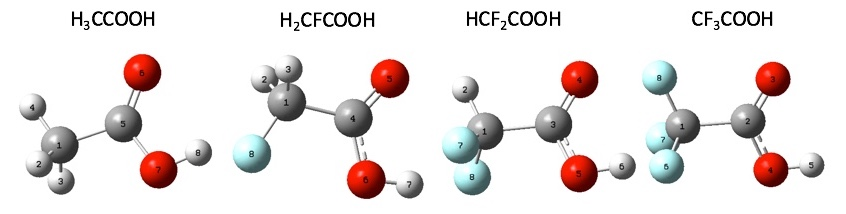
\includegraphics[scale=0.4]{grupo-COOH}
	\caption{Ácidos carboxílicos con diferentes sustituciones de hidrógenos por átomos de flúor.}
\end{figure}
\begin{figure}[H]
\centering
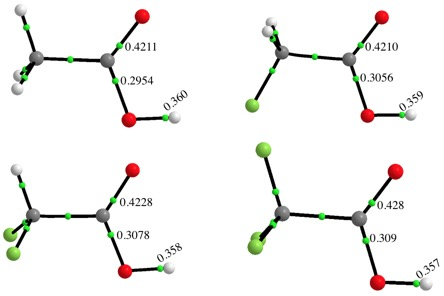
\includegraphics[scale=0.6]{AIM-CH3COOH}\cite{AIM}
\caption{Máximos de densidad de enlace.}
\end{figure}

Como se ven en la figura 3.8 a medida que aumentamos el número de átomos de flúor, disminuye la densidad electrónica debido a que, como se ha dicho antes, el flúor es un grupo atractor, el enlace O-H se debilita facilitando su ruptura, traduciéndose esto en un aumento de su acidez.
\begin{table}[H]
    \centering
    \begin{tabular}{|c|c|c|c|c|c|c|c|}
    \hline
    $CF_3-$ & Carga Nat. & $HCF_2-$ & Carga Nat. & $H_2CF-$ & Carga Nat.l  & $H_3C-$ & Carga Nat. \\ \hline
     C & 1.01480 &  C & 0.51364 & C & -0.00147 & C & -0.68072 \\ \hline
     C & 0.72404 &  H & 0.21440 & H & 0.18224 & H & 0.22348 \\ \hline
     O & -0.53625 & C & 0.73986 & H & 0.18224 & H & 0.22348 \\ \hline
     O & -0.66183 & O & -0.57168 & C & 0.78381 & H & 0.21946 \\ \hline
     H & 0.48893 & O & -0.69699 & O & -0.59271 & C & 0.82796 \\ \hline
     F & -0.34630 & H & 0.52359 & O & -0.66617 & O & -0.59224 \\ \hline
     F & -0.34629 & F & -0.36121 & H & 0.47979 & O & -0.69688 \\ \hline
     F & -0.33709 & F & -0.36161 & F & -0.36772 & H & 0.47546 \\ \hline
    \end{tabular}
    \caption{Carga Natural de moléculas con el grupo carboxi}
\end{table}

Como en los ácidos orgánicos, en los oxoácidos al sustituir un hidrógeno por un flúor también aumenta la acidez de la molécula, si nos fijamos en la tabla 3.7 situada al inicio de esté apartado, comprobamos que la molécula $HFCO_3$ es más ácida que el $H_2CO_3$, como hemos dicho antes por el efecto inductivo del flúor, ya que es un grupo atractor, en el caso de sustituir el hidrógeno por un cloro, pasa exactamente lo mismo, aumenta la acidez debido a su electronegatividad, pero ésta es menor si lo comparamos con la molécula con flúor ya que el cloro es menos electronegativo, pasa lo mismo en el caso del $H_2SO_4$, por otro lado, cuando añades HF a dicho ácido, también aumenta la acidez (ver FHSO3) por el mismo motivo.\\
{\bfseries con el fosfórico pasa al reves, como puede ser!!! }
\subsection{Hidratación específica}
Se estudia el impacto que tiene poner una molécula de agua en el sitio activo de los ácidos anteriormente estudiados en la acidez en fase gas, en la tabla \ref{tab:3.7} también se indica los valores de acidez en presencia de la molécula de agua en el sitio ácido.\\
A la vista de los resultados expuestos, la acidez aumenta al haber una molécula de agua en el punto acídico, debido a la formación de enlaces de hidrógeno fuertes como se verifica observando la existencia de máximos de densidad en dichos enlaces en la figura 3.9, y mirando las distancias d(O···H)  en la tabla 3.11.

\begin{figure} [H]
	\centering
	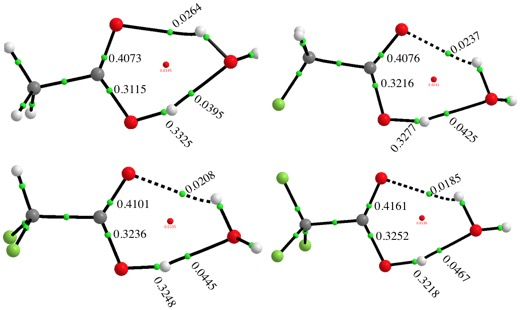
\includegraphics[scale=0.6]{AIM-CH3COOH-H2O}\cite{AIM}
	\caption{Máximos de densidad de enlace}
\end{figure}

 En este punto hay que tener en cuenta la donación de electrones $\sigma$ por parte del ácido a la molécula de agua y la retrodonación $\pi$ por parte de los pares libres del oxígeno de la molécula de agua.


{\bfseries TENGO QUE MIRAR DETENIDAMENTE EL H3PO4 Y H3PO4-H2O}

\begin{table}[H]
	\centering
	\begin{tabular}{|c|c|c|c|}
		\hline
		Ácidos-$H_2O$ & distancia	& d(O$\cdots$H) ($\Armstrong$) & $Max_{densidad, BPC} (u. a.)$ \\ \hline
		$CF_3COOH-H_2O$ & $d(O_9-H_5)$ &1,693&0,04665\\ \cline{2-4}
& $d(O_3-H_{10})$ & 2,137 & 0,01852 \\ \hline
 $CF_3COSH-H_2O$ & $d(O_9-H_8)$	 & 1,923 & 0,03014 \\ \cline{2-4}
	& $d(O_3-H_{10})$ & 2,049 & 0,02064 \\ \hline
	$CF_3SO_3H-H_2O$ & $d(O_{10}-H_4)$ & 1,614 & 0,05653 \\ \cline{2-4}
	& $d(O_5-H_{12})$	& 2,191 &	0,01631 \\ \hline
 $FHSO_3-H_2O$	& $d(O_7-H_4)$ & 1,610 &	0,05682 \\ \cline{2-4}
	& $d(O_5-H_8)$	& 2,313	& 0,01323 \\ \hline
 $H_2CFCOOH-H_2O$	&$d(O_9-H_7)$ & 1,735	& 0,04251 \\ \cline{2-4}
	& $d(O_5-H_{11})$ & 2,012	& 0,02375 \\ \hline
 $H_2CFCOSH-H_2O$ &	$d(O_3-H_{10})$ & 1,985 &	0,02356 \\ \cline{2-4}
	& $d(O_9-H_6)$ & 1,990	& 0,02633 \\ \hline
 $H_2CFSO_3H-H_2O$ &	$d(O_{10}-H_4)$	& 1,649	& 0,05205 \\ \cline{2-4}
	& $d(O_5-H_{11})$ & 2,079	& 0,02015 \\ \hline
 $H_2CO_3-H_2O$	& $d(O_7-H_5)$	& 1,737	& 0,04163 \\ \cline{2-4}
	& $d(O_2-H_9)$ & 2,201	& 0,01575 \\ \hline
 $H_2S_2O_6-H_2O$ &	$d(O_{11}-H_{10})$	& 1,548 &	0,06753 \\ \cline{2-4}
	& $d(O_2-H_{12})$ & 2,048 &	0,01959 \\ \hline
 $H_2SO_4-H_2O$	& $d(O_8-H_5)$ & 1,651	& 0,05181 \\ \cline{2-4}
	& $d(O_6-H_9)$ & 2,146	& 0,01768 \\ \hline
 $H_3CCOOH-H_2O$ & $d(O_9-H_8)$ & 1,767	& 0,03947 \\ \cline{2-4}
	& $d(O_6-H_{10})$ & 1,961 &	0,02645 \\ \hline
 $H_3CCOSH-H_2O$ &	$d(O_3-H_{10})$	& 1,958 &	0,02496 \\ \cline{2-4}
	& $d(O_9-H_5)$	& 2,000	& 0,02587 \\ \hline
 $H_3CSO_3H-H_2O$	& $d(O_{10}-H_4)$	& 1,689	& 0,04736 \\ \cline{2-4}
	& $d(O_5-H_{11})$	& 2,065 &	0,02080 \\ \hline
 $HCF_2COOH-H_2O$	& $d(O_9-H_6)$	&1,715	& 0,04446 \\ \cline{2-4}
	& $d(O_4-H_{11})$ & 2,078	& 0,02083 \\ \hline
 $HCF_2COSH-H_2O$	& $d(O_9-H_7)$ &1,949 & 0,02858 \\ \cline{2-4}
	& $d(O_3-H_{10})$ & 2,021 &	0,02186 \\ \hline
 $HCF_2SO_3H-H_2O$	& $d(O_{10}-H_4)$ & 1,634	& 0,05386 \\ \cline{2-4}
&	$d(O_5-H_{12})$ & 2,110	& 0,01899 \\ \hline
 $HPO_3-H_2O$	& $d(O_6-H_2)$ & 1,659	& 0,05063 \\ \cline{2-4}
	& $d(O_4-H_7)$ & 2,103	& 0,01920 \\ \hline
 $HNO_3-H_2O$	& $d(O_6-H_2)$	& 1,677	& 0,04803 \\ \cline{2-4}
	& $d(O_4-H_7)$ & 2,261	& 0,01515 \\ \hline
	\end{tabular}
\caption{Análisis de enlaces de hidrógeno en los ácidos objeto de estudio.}
\end{table}
\begin{figure}[H]
	\centering
	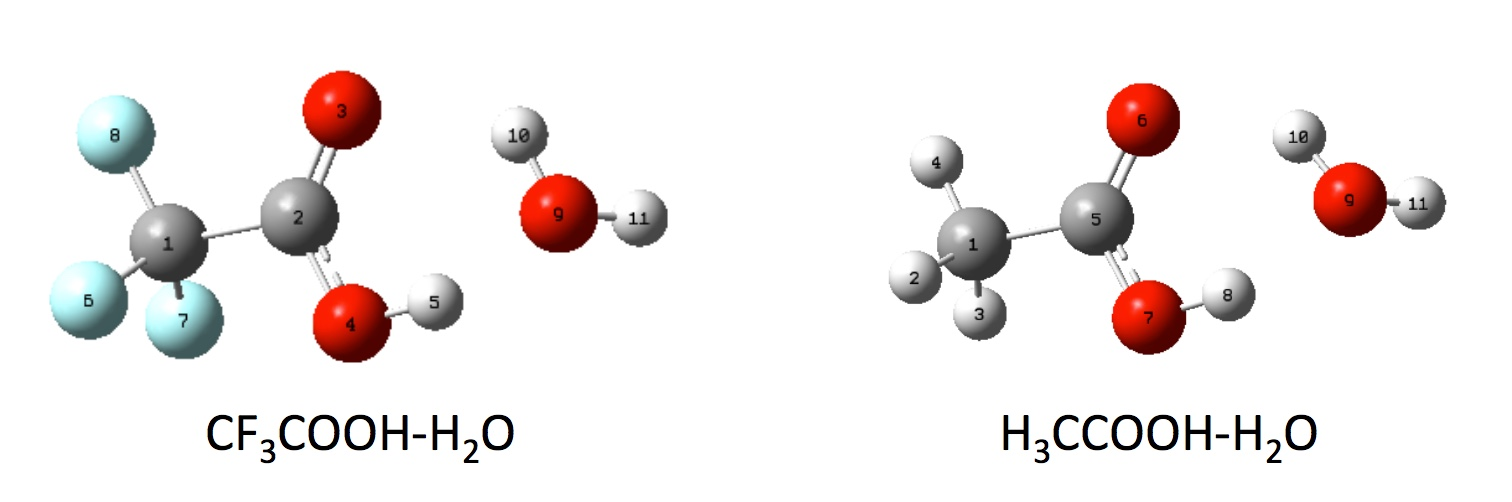
\includegraphics[scale=0.2]{acidos-h2o}
	\caption{Ácidos-$H_2O$}
\end{figure}
 Teniendo en cuenta el análisis NBO de dichas moléculas también se confirma la mayor facilidad para romper el enlace O-H cuando se expone el punto activo del ácido a una molécula de agua.
 
 La retrodonación y donación electrónica es la energía de deslocalizacion orbitalaria de los componentes de un complejo, es decir, a mayor donación y retrodonación mayor energía.
 
 En la molécula $H_3CCOOH$, los dos pares libres de electrones del átomo $O_7$ donan electrones a orbitales antienlazantes del $C_5=O_6$, esta donación se traduce en forma de energía a 5,69 y 44,35 Kcal/mol,  mientras que en la molécula de $H_3COOH-H_2O$, al formar un enlace de hidrógeno, la donación por parte de los pares de electrones libres del $O_7$ energéticamente se traduce en 7,28 y 53,66 Kcal/mol , por lo que el enlace O-H se debilita, y en consecuencia aumenta la acidez de dicha molécula.
 
 La diferencia de acidez entre el $CF_3COOH$ y el $H_3CCOOH$ es de 24,53 Kcal/mol, y la diferencia en las mismas moléculas, hidratadas ($CF_3COOH-H_2O$ y $H_3CCOOH-H_2O$) tiene un valor de 19,89 Kcal/mol. Esto lleva a pensar que el efecto del agua  en el ácido trifluoretanoico, no es completo, puesto que el efecto inductivo del los tres halógenos compite con éste. En el caso del ácido etanoico, al no tener efecto inductivo por parte de ninugún halógeno, sino que tiene un $CH_3$, dador de densidad electrónica,  el incremento de la acidez de dicho ácido hidratado es mayor.
 Se ven algunas de las distancias de dichos ácidos en la tabla 3.12.
 \begin{table}[H]
 	\centering
 	\begin{tabular}{|c|c|c|c|c|c|c|}
 		\hline
 			 & d(C-F)	& d(O-H) & d(C=O) & & d(O-H) & d(C=O) \\ \hline
$CF_3COOH$ & 1,340 & 0,970 & 1,190 & $H_3CCOOH$ & 0,969 &1,210 \\ \hline $CF_3COOH-H_2O$	& 1,340 & 0,999 & 1,210 & $H_3CCOOH-H_2O$	& 0,991 &1,220 \\ \hline
 	\end{tabular}
 \caption{Distancias internucleares de interés de cada ácido en $\Armstrong$}
 \end{table}

Con el análisis NBO se muestra que  hay una donación del par de electrones libre del $O_9$ de la molécula de $CF_3COOH-H_2O$ al enlace $O_4-H_5$, esa donación se traduce en  24,26 Kcal/mol de energía, no hay prácticamente retrodonación por parte del $O_4-H_5$, 0,06 Kcal/ mol. En la molécula $H_3COOH-H_2O$, $O_9$ dona el par de electrones al enlace $O_7-H_8$ ()18,59 Kcal/mol de energía), en este caso la retrodonación es nula por parte del enlace $O_7-H_8$. La donación por uno de los pares de electrones libres de los átomos de oxígeno $O_4$ y $O_7$  de las moléculas $CF_3COOH-H_2O$ y $H_3CCOOH-H_2O$ respectivamente, a los enlaces C=O correspondientes, es mayor en el ácido $CF_3COOH-H_2O$ que en el $H_3CCOOH-H_2O$, traduciéndose esto en una mayor acidez del primer complejo.
